%%%%%%%%%%%%%%%%%%%%%%%%%%%%%%%%%%%%%%%%%
% Stylish Article
% LaTeX Template
% Version 2.1 (1/10/15)
%
% This template has been downloaded from:
% http://www.LaTeXTemplates.com
%
% Original author:
% Mathias Legrand (legrand.mathias@gmail.com) 
% With extensive modifications by:
% Vel (vel@latextemplates.com)
%
% License:
% CC BY-NC-SA 3.0 (http://creativecommons.org/licenses/by-nc-sa/3.0/)
%
%%%%%%%%%%%%%%%%%%%%%%%%%%%%%%%%%%%%%%%%%

%----------------------------------------------------------------------------------------
%	PACKAGES AND OTHER DOCUMENT CONFIGURATIONS
%----------------------------------------------------------------------------------------

\documentclass[fleqn,10pt]{SelfArx} % Document font size and equations flushed left

\usepackage{lipsum} % Required to insert dummy text. To be removed otherwise
\usepackage{csvsimple}
%----------------------------------------------------------------------------------------
%	COLUMNS
%----------------------------------------------------------------------------------------

\setlength{\columnsep}{0.55cm} % Distance between the two columns of text
\setlength{\fboxrule}{0.75pt} % Width of the border around the abstract

%----------------------------------------------------------------------------------------
%	COLORS
%----------------------------------------------------------------------------------------

\definecolor{color1}{RGB}{0,0,90} % Color of the article title and sections
\definecolor{color2}{RGB}{0,20,20} % Color of the boxes behind the abstract and headings
\usepackage[italian]{babel} 
%----------------------------------------------------------------------------------------
%	HYPERLINKS
%----------------------------------------------------------------------------------------

\usepackage{hyperref} % Required for hyperlinks
\hypersetup{hidelinks,colorlinks,breaklinks=true,urlcolor=color2,citecolor=color1,linkcolor=color1,bookmarksopen=false,pdftitle={Title},pdfauthor={Author}}

%----------------------------------------------------------------------------------------
%	ARTICLE INFORMATION
%----------------------------------------------------------------------------------------

\JournalInfo{Journal, Vol. XXI, No. 1, 1-5, 2013} % Journal information
\Archive{Additional note} % Additional notes (e.g. copyright, DOI, review/research article)


\PaperTitle{\center Progetto di Metodi statistici per l'apprendimento: K-Nearest Neighbors} % Article title
\Authors{\center \textbf{Studente:} Marco Odore - \textbf{Matricola:} 868906}
 % Authors

\Keywords{Apprendimento Supervisionato --- K-NN --- Classificazione binaria} % Keywords - if you don't want any simply remove all the text between the curly brackets
\newcommand{\keywordname}{Keywords} % Defines the keywords heading name

%----------------------------------------------------------------------------------------
%	ABSTRACT
%----------------------------------------------------------------------------------------

\Abstract{Implementzione in R e C++ dell'algoritmo K-nearest neighbors e sua applicazione ad un problema di classificazione binaria, nella sua versione classica e online.}

%----------------------------------------------------------------------------------------

\begin{document}

\flushbottom % Makes all text pages the same height

\maketitle % Print the title and abstract box

\tableofcontents % Print the contents section

\thispagestyle{empty} % Removes page numbering from the first page

%----------------------------------------------------------------------------------------
%	ARTICLE CONTENTS
%----------------------------------------------------------------------------------------

\section*{Introduzione} % The \section*{} command stops section numbering

\addcontentsline{toc}{section}{Introduction} % Adds this section to the table of contents

Si è scelto di implementare in R l'algoritmo di apprendimento supervisionato K-NN e di applicarlo ad un problema di classificazione binario, dove si vuole associare ad una persona il suo possibile reddito annuale (discretizzato, tramite una soglia, a due valori possibili), date alcune sue informazioni di base. 

\subsection{Il dataset}
Il dataset utilizzato \cite{Lichman:2013} contiene 48842 istanze, ognuna delle quali è caratterizzata da 14 feature:

\begin{itemize}
\footnotesize{
\item \textbf{Età} - Tipo continuo
\item \textbf{Workclass} - Tipo nominale (8 valori possibili)
\item \textbf{Fnlwgt} - Tipo continuo
\item \textbf{Education} - Tipo nominale (16 valori possibili)
\item \textbf{Education-num} - Tipo continuo (trasformazione di education in tipo continuo)
\item \textbf{Marital-status} - Tipo nominale (7 valori possibili)
\item \textbf{Occupation} - Tipo nominale (14 valori possibili)
\item \textbf{Relationship} - Tipo nominale (6 valori possibili)
\item \textbf{Race} - Tipo nominale (6 valori possibili)
\item \textbf{Sex} - Tipo nominale (2 valori possibili)
\item \textbf{Capital-gain} - Tipo continuo 
\item \textbf{Capital-loss} - Tipo continuo
\item \textbf{Hours-per-week} - Tipo continuo
\item \textbf{Native-country} - Tipo nominale (41 valori possibili)}
\end{itemize}
Per rendere l'input gestibile da K-NN, si sono trasformate le feature di tipo nominale in una serie di feature binarie, e cioè utilizzando delle variabili dummy per ogni possibile valore che la feature può assumere\footnote{\footnotesize{Con l'introduzione delle variabili dummy si è passati a 88 feature complessive.}}.
\newline
Per quanto riguarda l'etichettatura, ognuna delle istanze può assumere due possibili valori, e cioè
\begin{itemize}
\item \textbf{classe 1}: $\le50k$
\item \textbf{classe 2}: $>50k$ 
\end{itemize} 

Il dataset risulta essere sbilanciato, in quanto la classe 2 rappresenta il $23.93\% $ del dataset (la classe 1 il $76.07\% $). Inoltre al suo interno vi sono alcune istanze che per alcune feature non possiede specificazioni. Per questa motivazione si è deciso di escluderle dal processo di valutazione ed apprendimento, riducendo così la cardinalità complessiva del dataset a 45222 istanze\footnote{\footnotesize{Senza le istanze con valori sconosciuti le percentuali delle classi 1 e 2 si attestano rispettivamente su $75.22\%$ e $24.78\%$.}}. 

\subsection{Ottimizzazione delle performance}
Data la lentezza dell'algoritmo K-NN, soprattutto con grandi dataset, si è deciso di implementare la funzione di ricerca per i k più vicini in C++, che rispetto ad R risulta molto più veloce. Per quanto riguarda il task di \emph{cross-validation} invece, si è deciso di parallelizzarlo grazie ad una funzione fornita da una libreria di R\footnote{\emph{parLapply}, nella libreria di R \emph{parallel}.}, che ha permesso di suddividere agevolmente il problema.



%------------------------------------------------

\section{Metodi e valutazione dei modelli}

Per il problema trattato si sono utilizzate due versioni di K-NN, e cioè quella classica e quella online.

\subsection{K-NN}
Questo algoritmo permette di generare un classificatore $h_{k-NN}$ memorizzando l'intero training set fornito in input e calibrando un suo parametro $k$, il quale permette di gestire l'underfitting e l'overfitting sul problema.
\newline
\newline
L'assegnazione dell'etichetta ad un'istanza $x$ avviene nella seguente maniera:
\newline
\newline
\textbf{$h_{k-NN}(x)=$}la maggioranza delle etichette $y_t$ delle $k$ istanze $x_t$ più vicine a $x$

\subsection{K-NN online}
Si tratta di una variante di K-NN che in fase di training opera nella seguente maniera:
\begin{itemize}
\item Prova a classificare l'istanza $x_t$ usando K-NN sull'insieme $S$.
\item Se $h_{K-NN}(x_t)\neq y_t$ aggiungi $x_t$ all'insieme $S$.
\end{itemize}


L'algoritmo inizia da un insieme $S$ vuoto, aggiungendovi man mano esempi quando sbaglia, lasciandolo inalterato invece quando non commette errori.

\subsection{Nested Cross-Validation}
Per la stima delle performance dei classificatori generati dalla versione base di K-NN e quella online si è deciso di utilizzare la \emph{cross-validation esterna} a 5 fold, sfruttando come metrica il \emph{test error}, calcolato come segue:

\[\widetilde{er}(h_{k-NN})=\frac{1}{n}\sum_{i=1}^{n} l(y_t,h_{k-NN}(x_t))\]

Dove $l$ è la funzione di perdita \emph{zero-uno}, che vale 1 nel caso in cui il predittore commette un errore, 0 altrimenti.
\newline

Per selezionare invece il $k$ ottimale automaticamente, si è effettuata una cross-validation interna, sempre a 5 fold, sia nella fase di selezione finale (dove viene scelto il $k$ finale del modello), sia per la selezione del $k$ ottimale di ogni singolo fold generato dalla cross validazione esterna. Nella figura \ref{cross} sono mostrati i passi della \emph{nested cross-validation} (cross validazione interna + cross validazione esterna)
\begin{figure}
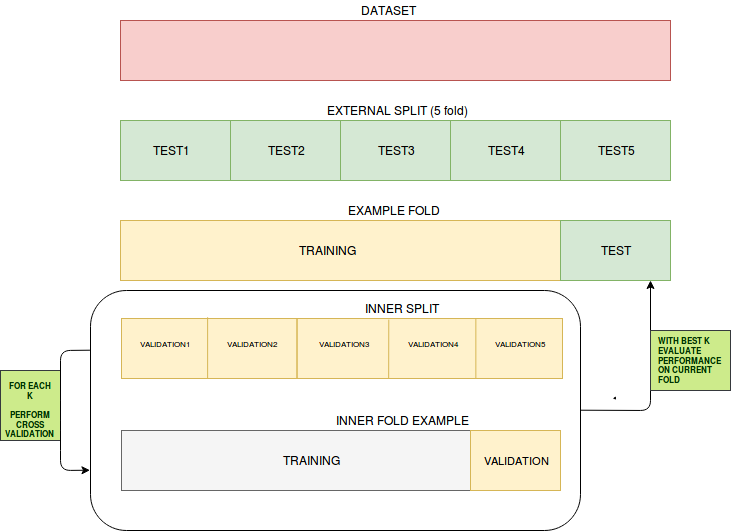
\includegraphics[scale=0.33]{cross.png}
\caption{\footnotesize{Il modo in cui è avvenuto lo split del dataset sia per la cross validazione esterna (split più esterno) sia per la cross validazione interna (split interno sui singoli training set di ogni rispettivo fold)}}
\label{cross}
\end{figure}

\subsection{Rischio sequenziale}
Nel caso specifico di K-NN online si è deciso inoltre di valutare l'andamento del rischio sequenziale sull'intero dataset, calcolato come segue:

\[
er_{seq}(t)=\frac{1}{t}\sum_{i=1}^{t} l(y_t,h_{k-NN}(x_t))
\]

ad ogni passo t, e cioè alla t-esima istanza fornita in pasto all'algoritmo.
\section{Sperimentazione e analisi}
La sperimentazione è stata effettuata sia normalizzando i dati\footnote{\footnotesize{Ogni specificazione delle feature è stata trasformata in una specificazione di una normale standard, sottraendo ad ogni valore la media campionaria e dividendo per la deviazione standard campionaria}}, sia in assenza di normalizzazione, questo per verificare l'impatto che questa procedura ha sulle performance dei classificatori generati.
\newline
\newline
La ricerca del parametro $k$ è avvenuta su di un set di 26 possibili valori\footnote{\footnotesize{K=\{1, 3, 5, 7, 9, 11, 13, 15, 17, 19, 21, 23, 25, 27, 29, 31, 33, 35, 37, 39, 41, 43, 45, 47, 49, 51\}}}.

\subsection{K-NN senza normalizzazione}
Le curve del test error al variare di k, valutate tramite cross-validation interna per ogni fold, hanno un andamento molto simile, come si evince dalla figura \ref{cross:int1}.
\begin{figure}
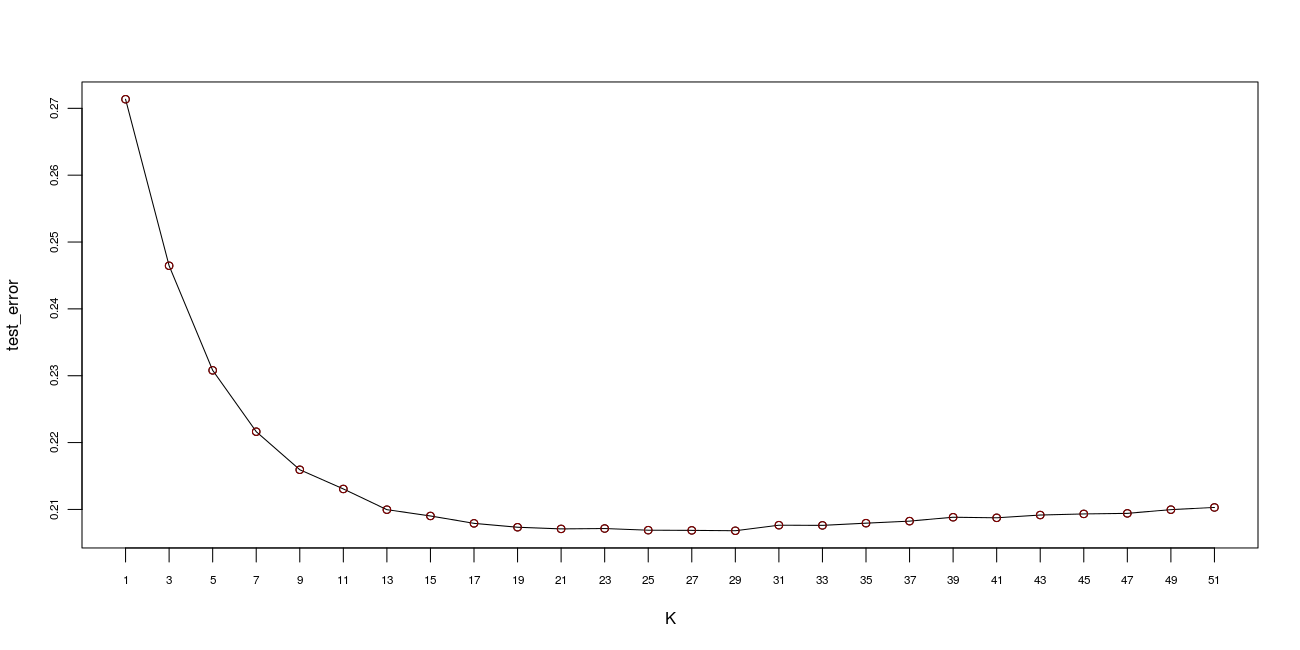
\includegraphics[scale=0.27]{knn_wo_norm/fold_1.png}
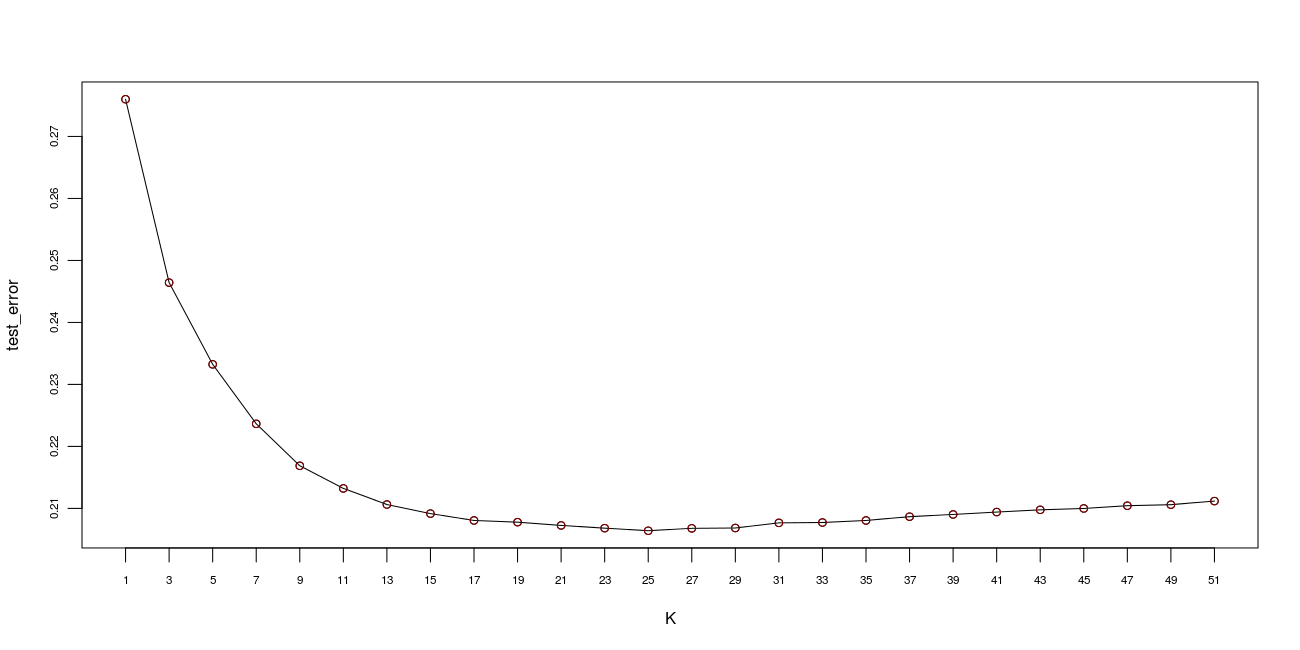
\includegraphics[scale=0.27]{knn_wo_norm/fold_2.png}
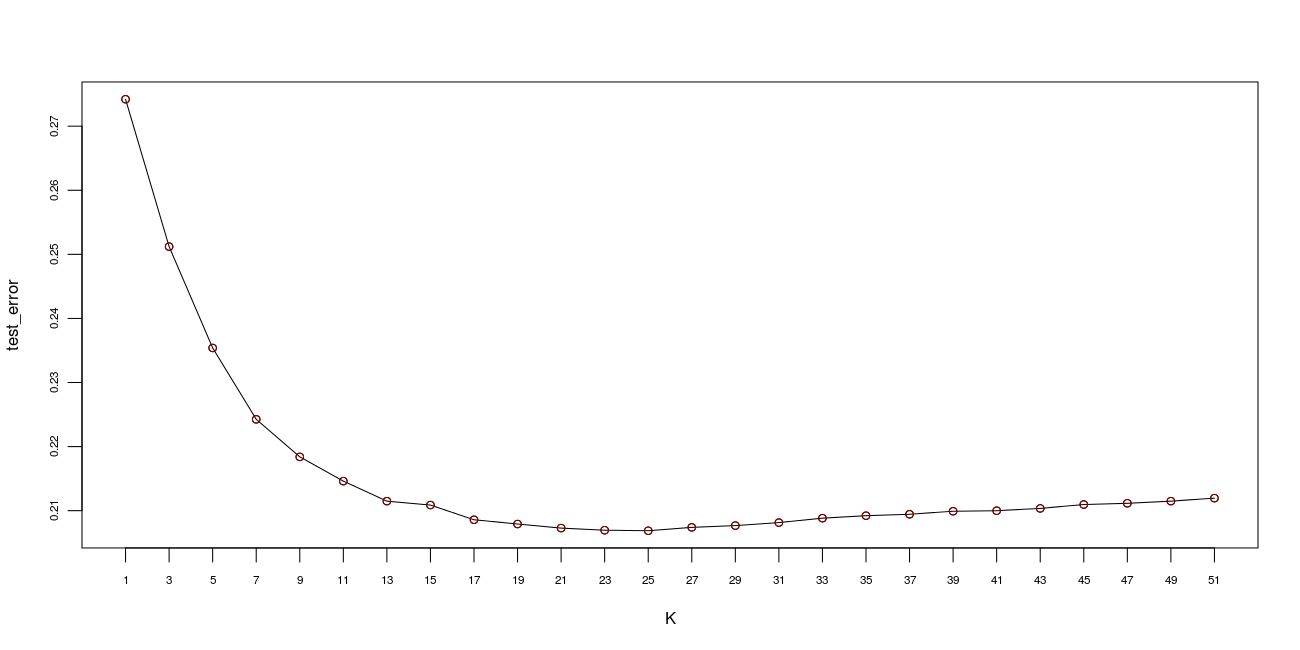
\includegraphics[scale=0.27]{knn_wo_norm/fold_3.png}
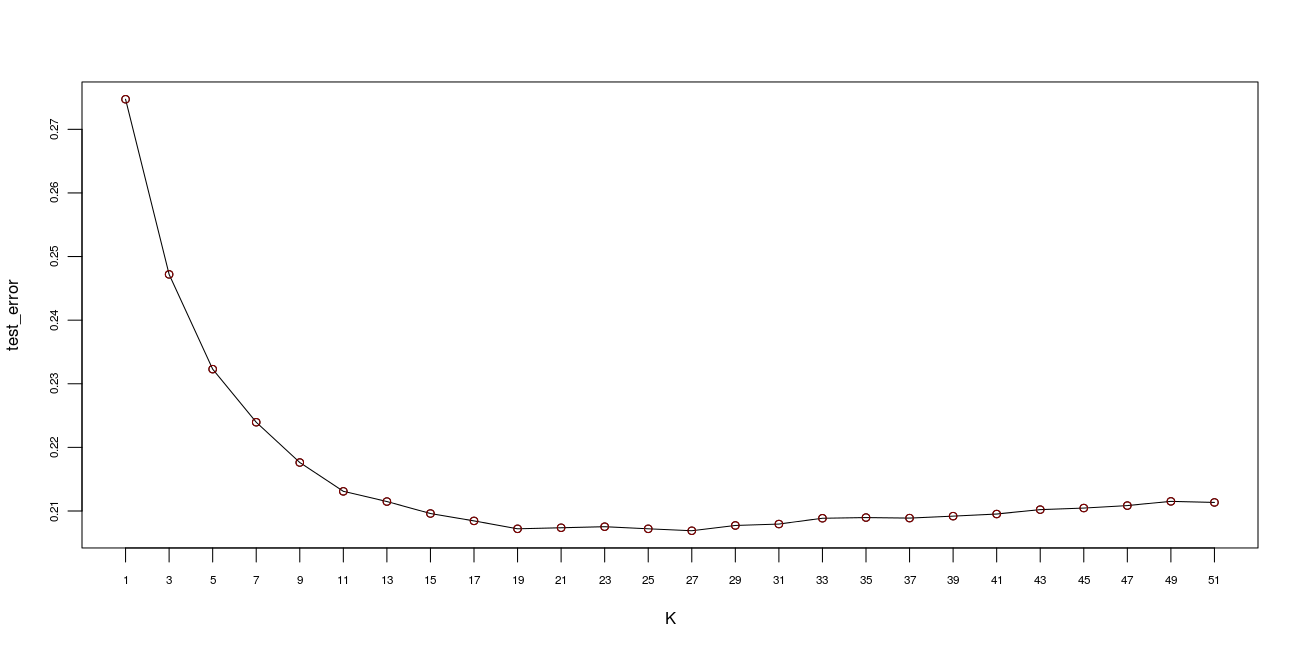
\includegraphics[scale=0.27]{knn_wo_norm/fold_4.png}
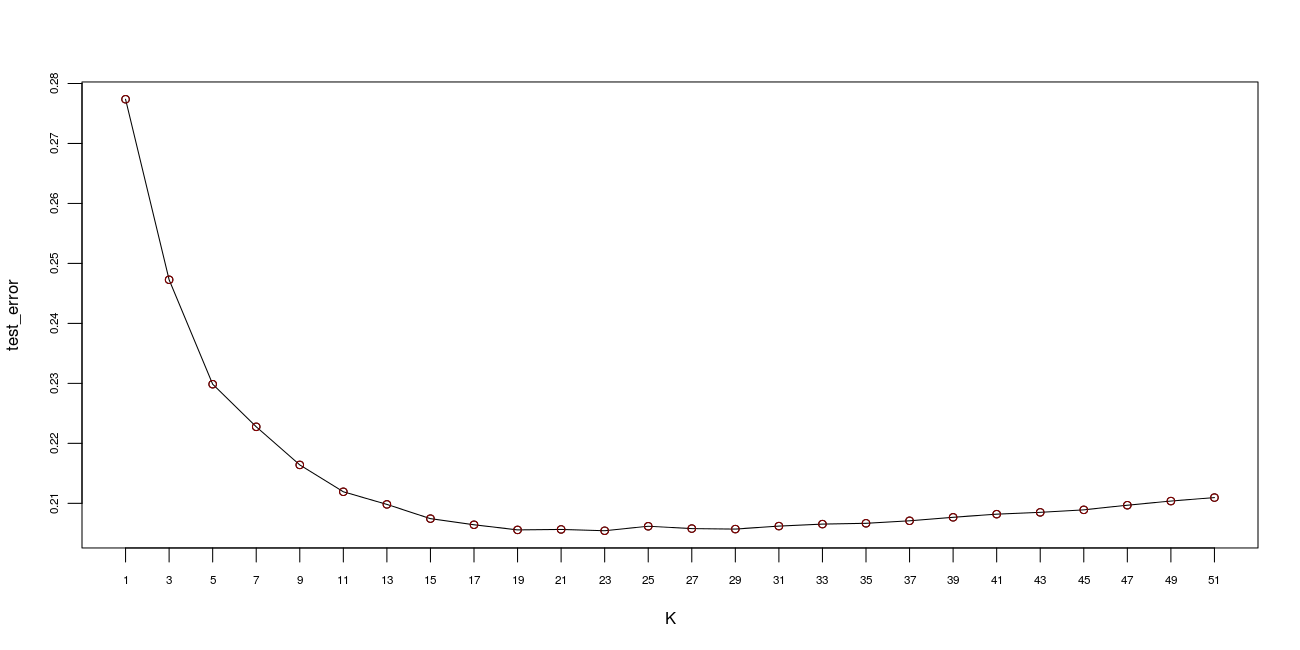
\includegraphics[scale=0.27]{knn_wo_norm/fold_5.png}
\caption{\footnotesize{Test error (della cross validazione interna al fold) al variare di $k$ per ogni singolo fold.}}
\label{cross:int1}
\end{figure}
\newline
\newline
Il test error ha infatti il classico comportamento che si può osservare in K-NN, e cioè diminuisce progressivamente fino ad arrivare ad un $k^{*}$ ottimo in cui l'errore è minimo, per poi ritornare a salire nuovamente. I $k^{*}$ ottimi ottenuti risultano essere poi relativamente vicini per ogni fold (così come il test error), come si evince dalla tabella \ref{cross:k1}.
\newline
\begin{table}
\center
\begin{tabular}{l|l|l|l|l|l}%
    \bfseries  fold & \bfseries k % specify table head
    \csvreader[head to column names]{knn_wo_norm/k.csv}{}% use head of csv as column names
    {\\\hline \csvcoli&\csvcolii}% specify your coloumns here
    \end{tabular}
    \caption{\footnotesize{I k ottimi generati per ogni fold.}}
    \label{cross:k1}
\end{table}

La performance finale del classificatore con selezione automatica del $k^{*}$ ottimo, valutata con cross validazione esterna, si attesta sul $79\% $ di accuratezza. Infine è stato selezionato il k finale del modello, con una nuova cross validation interna, questa volta su tutto il dataset, che è risultato essere pari a 25. L'andamento del test error al variare di k sulla cross-validation interna finale, è mostrata nella figura \ref{cross:final1}. 
\begin{figure}
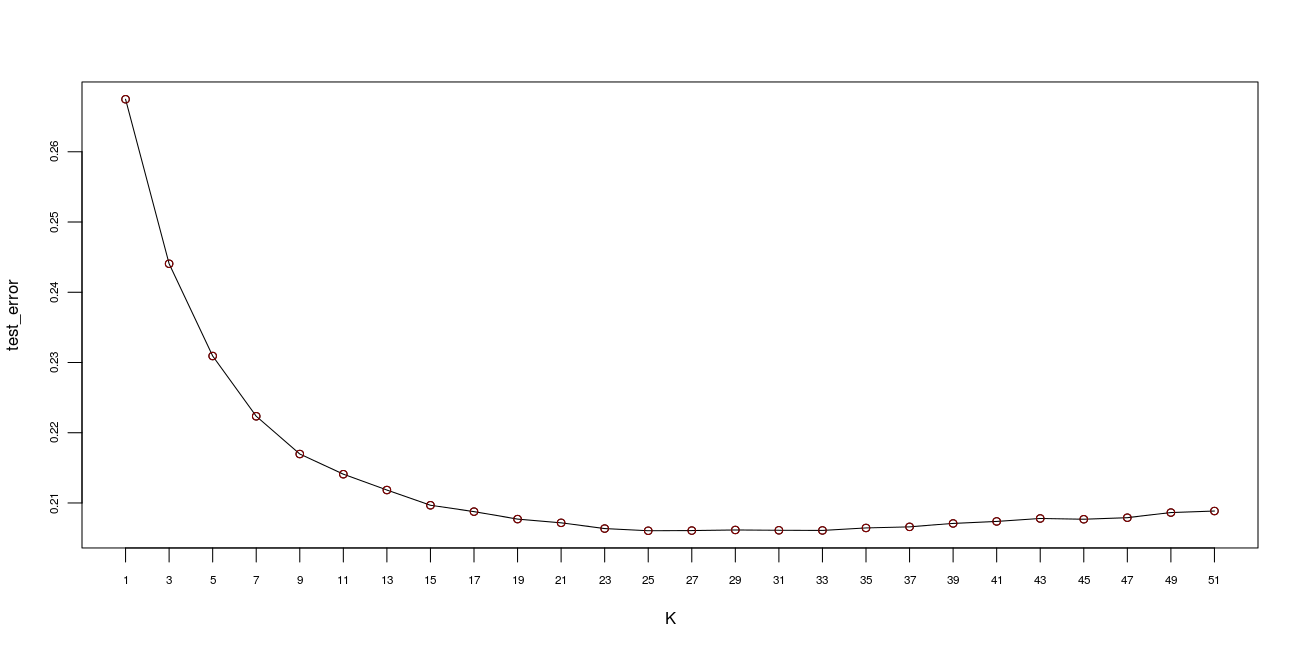
\includegraphics[scale=0.27]{knn_wo_norm/final.png}
\caption{\footnotesize{Test error al variare di $k$ per la cross validazione interna finale.}}
\label{cross:final1}
\end{figure}
\newline
\newline
Nelle tabelle \ref{cross:prec1} e \ref{cross:stats1} vi sono un po' di statistiche dettagliate su questa specifica sperimentazione.
\begin{table}
\center
\begin{tabular}{l|l|l}%
    \bfseries  class & \bfseries precision % specify table head
    \csvreader[head to column names]{knn_wo_norm/prec.csv}{}% use head of csv as column names
    {\\\hline \csvcoli&\csvcolii}% specify your coloumns here
    \end{tabular}
    \caption{\footnotesize{La precision finale per le due classi.}}
 	\label{cross:prec1}
 \end{table}
 \begin{table}
 \center
    \begin{tabular}{l|l|l}%
    \bfseries  time & \bfseries accuracy & \bfseries finalK % specify table head
    \csvreader[head to column names]{knn_wo_norm/stats.csv}{}% use head of csv as column names
    {\\\hline \csvcoli&\csvcolii&\csvcoliii}% specify your coloumns here
    \end{tabular}
    \caption{\footnotesize{Alcune statistiche della sperimentazione. Il tempo totale per effettuare la nested cross-validation, espresso in secondi, l'accuratezza finale +- deviazione standard e il k finale selezionato.}}
    \label{cross:stats1}
\end{table}
\subsection{K-NN con normalizzazione dei dati}
A seguito della normalizzazione dei dati, i $k^{*}$ ottimi generati per ogni fold, a seguito della cross validazione interna, risultano essere tutti inferiori ai $k^{*}$ ottimi generati dal dataset non normalizzato, come si evince dalla tabella \ref{cross:k2}. 
\newline
\begin{table}
\center
\begin{tabular}{l|l|l|l|l|l}%
    \bfseries  fold & \bfseries k % specify table head
    \csvreader[head to column names]{knn_norm/k.csv}{}% use head of csv as column names
    {\\\hline \csvcoli&\csvcolii}% specify your coloumns here
    \end{tabular}
    \caption{\footnotesize{I k ottimi generati per ogni fold, dal dataset normalizzato.}}
    \label{cross:k2}
\end{table}

Inoltre il test error medio risultato della cross-validazione esterna risulta essere inferiore (accuratezza dell'83\%). Vi è però un netto calo della precision per la classe 2, a differenza della classe 1, che invece sembra guadagnare molto dalla normalizzazione, come si può notare dalla tabella \ref{cross:prec2} (confronto con tabella \ref{cross:prec1}). 

\begin{table}
\center
\begin{tabular}{l|l|l}%
    \bfseries  class & \bfseries precision % specify table head
    \csvreader[head to column names]{knn_norm/prec.csv}{}% use head of csv as column names
    {\\\hline \csvcoli&\csvcolii}% specify your coloumns here
    \end{tabular}
    \caption{\footnotesize{La precision finale per le due classi, per il dataset normalizzato.}}
 	\label{cross:prec2}
 \end{table}
 
 Infine il $k^{*}$ ottimo selezionato con la cross-validazione interna finale applicata all'intero dataset è risultato essere 31. L'andamento del test error medio per la selezione del parametro ottimale, al variare di k, è mostrato nella figura \ref{cross:final2}. Nella tabella \ref{cross:stats2} vi sono delle statistiche relative a questa specifica sperimentazione.
 \newline
 
 \begin{figure}
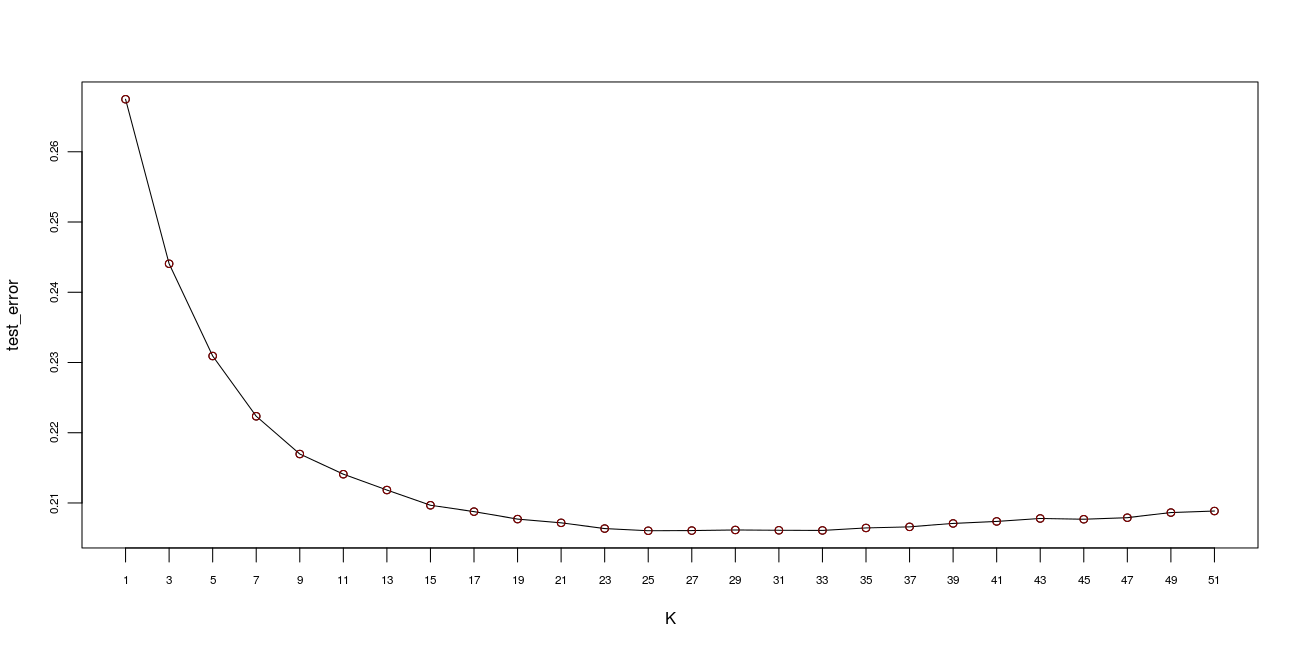
\includegraphics[scale=0.27]{knn_wo_norm/final.png}
\caption{\footnotesize{Test error al variare di $k$ per la cross validazione interna finale, per il dataset normalizzato.}}
\label{cross:final2}
\end{figure}
 \begin{table}
 \center
    \begin{tabular}{l|l|l}%
    \bfseries  time & \bfseries accuracy & \bfseries finalK % specify table head
    \csvreader[head to column names]{knn_norm/stats.csv}{}% use head of csv as column names
    {\\\hline \csvcoli&\csvcolii&\csvcoliii}% specify your coloumns here
    \end{tabular}
    \caption{\footnotesize{Alcune statistiche della sperimentazione con normalizzazione del dataset. Il tempo totale per effettuare la nested cross-validation, espresso in secondi, l'accuratezza finale +- deviazione standard e il k finale selezionato.}}
    \label{cross:stats2}
\end{table}


Nel complesso, la standardizzazione ha effettivamente apportato delle variazioni di performance, anche se non totalmente positivo, come si evince dall'aumento dei falsi positivi per la classe 2. 

\subsection{K-NN Online senza normalizzazione}

Passando all'analisi dell'algoritmo online, si è comunque cercato di selezionare un $k^{*}$ ottimale, automaticamente, tramite cross-validazione interna sull'intero dataset, applicando per ogni test set K-NN base e usando l'insieme S generato da ogni singolo training set dello split.
\newline

Come si può notare dalla figura \ref{cross:final3}, in questo caso l'andamento del test error al variare di k è molto più irregolare rispetto alla versione non online dell'algoritmo, e segue dei bruschi cambiamenti di direzione. Questo è giustificato dal fatto che in fase di learning l'insieme S generato da ogni training set della cross-validation interna può cambiare anche radicalmente come contenuto (a causa della variabile k), e quindi può portare a risultati nettamente differenti in fase di valutazione sul validation set. Il $k^{*}$ ottimo è risultato essere 19.

\begin{figure}
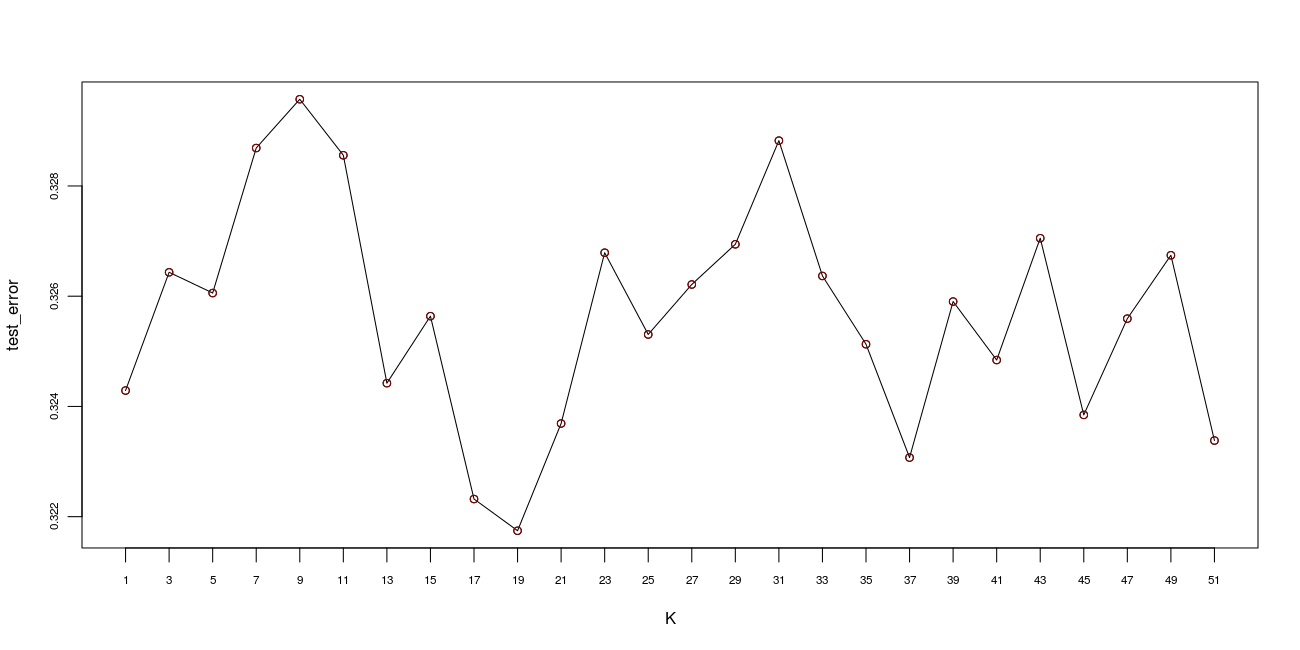
\includegraphics[scale=0.27]{knn_online_wo_norm/final_seq.png}
\caption{\footnotesize{Test error per K-NN online, al variare di $k$ per la cross validazione interna finale. Dataset non normalizzato.}}
\label{cross:final3}
\end{figure}

Per quanto riguarda l'analisi del rischio sequenziale, calcolato sull'intero dataset, utilizzando come k il $k^{*}$ ottimo selezionato precedentemente, questo descresce molto rapidamente, fino a stabilizzarsi verso un test error di 0.33 (accuratezza del 67\%), come si può notare dalla figura \ref{cross:seqrisk}.

\begin{figure}
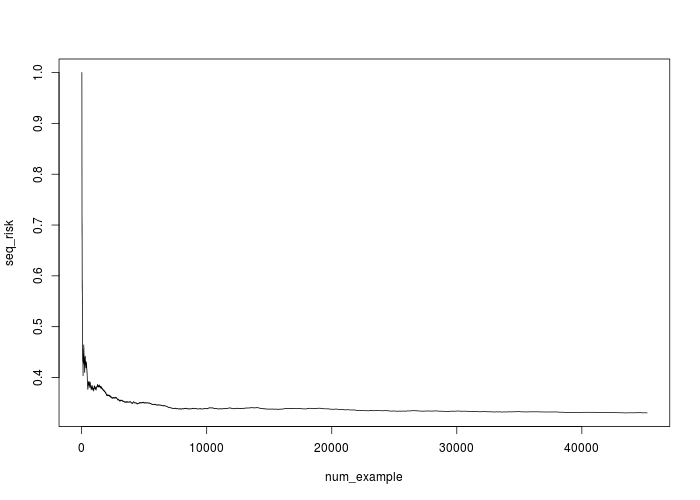
\includegraphics[scale=0.35]{knn_online_wo_norm/seq_risk_final.png}
\caption{\footnotesize{Rischio sequenziale con k = 19. Il rischio decresce dopo pochissimi esempi verso valori tra lo 0.33 e 0.40}}
\label{cross:seqrisk}
\end{figure}
Come conseguenza, si può notare dalla figura \ref{cross:misclass} come a cardinalità dell'insieme S cresca linearmente con l'arrivo di nuovi esempi, arrivando a contenere un totale di 14942 istanze (il 33\% dell'intero dataset, che è anche il valore del test error finale).

\begin{figure}
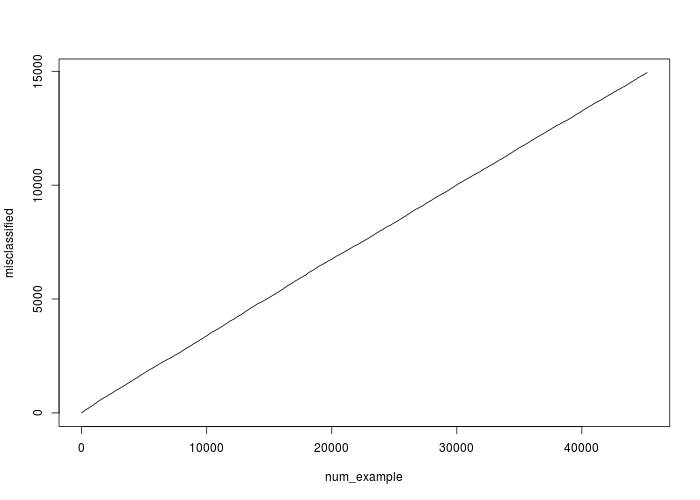
\includegraphics[scale=0.30]{knn_online_wo_norm/misclassified_final.png}
\caption{\footnotesize{Cardinalità dell'insieme S (ordinate) con l'arrivo dei nuovi esempi (ascisse). Dataset non normalizzato.}}
\label{cross:misclass}
\end{figure}

\section{Lavori futuri}
\begin{itemize}
\item Introduzione di altre metriche per la valutazione, come la Recall, la F-measure e la AUC per la curva ROC.
\item Verifica delle performance a seguito dello shuffling dei dati.
\item Verifica delle performance su diversi sub-set di feature.
\item Applicazione di diversi metodi di normalizzazione delle feature (ad esempio normalizzazione nel range [0,1], oppure normalizzazione al vettore unitario).

\end{itemize}

%----------------------------------------------------------------------------------------
%	REFERENCE LIST
%----------------------------------------------------------------------------------------

\bibliography{article_3}
\bibliographystyle{unsrt}



%----------------------------------------------------------------------------------------

\end{document}